\chapter{Introduction}

Around 2008, \textbf{\acf{SDN}}\index{software-defined networking}
\cite{Casado:2005:VNS:1047344.1047383} emerged from research at
Berkeley\index{Berkeley} and
Stanford\index{Stanford} as a way to enable networks to be defined and managed using
software One model of \acs{SDN} is \textit{OpenFlow}\todo{Cite!}, which
decouples the control plane\index{control plane} from the forwarding
plane\index{forwarding plane}\index{data plane|see{forwarding plane}} in a
switch, moving it out to an external networking node.  It enables one to
implement the controller in software.

Although invented quite recently, software-defined networking is already
being heavily used both in academia and industry.  Google\index{Google}, for instance, are
using OpenFlow to ease deploymend and increase utilization in their backbone
networks\index{backbone network} \cite{crabbe2012sdn} and Stanford has deployed several
OpenFlow-controlled networks on their university network.

In March 2013, IDC\index{IDC} \todo{finn ut hva det står for} projected that the SDN market would
  reach \${}3.7 billion by 2016, capturing a 35\%{} share of the switching
  market \cite{Kirkpatrick:2013:SN:2500468.2500473}.
\todo{Skriv om denne setningen, den er tatt nesten direkte fra artikkelen!}

OpenFlow is detailed in chapter \ref{chapter:background.openflow}
\vpageref{chapter:background.openflow}.

\textbf{Paxos}\index{Paxos} \cite{Lamport:1998:PP:279227.279229} is a
family of distributed, fault-tolerant consensus algorithms.  It allows
network nodes to reach \textit{agreement} even in the face of intermittent
network failures.  For example, one can design a database system using Paxos
to make sure that transactions are executed in the same order on all nodes.

Originally published by Leslie Lamport\index{Lamport, Leslie} in 1989, Paxos
has spawned numerous extensions like Byzantine tolerance\index{Byzantine
tolerance} and so on.  It is discussed in chapter
\ref{chapter:background.paxos} \vpageref{chapter:background.paxos}.

\textbf{Our aim} is to build an efficient, \textit{Paxos-enabled software defined
network}.  Paxos will be implemented on OpenFlow switches to guarantee that
packets sent to all of their connected nodes are sent in the same order.
These end-hosts can run any networking service and leverage the benefits of
Paxos without needing to handle any details of the algorithm.

\section{Hypothesis}

For simplicity, we will constrain our scope to a few primitives of
non-Byzantine\index{non-Byzantine}, classic crash Paxos\index{Paxos!classic
crash}in \textit{phase two}, where we have steady-state
flow\index{Paxos!steady-state flow} with no failures\index{Paxos!failure}.

Furthermore, we want to look at opportunities for increasing networking
performance by moving parts of the Paxos from the control
plane\index{control plane} down to the switches' forwarding
plane\index{forwarding plane}.

We will implement this in progressive stages:

\begin{enumerate}
\item Implement Paxos entirely on an OpenFlow software controller.
\item Extend OpenFlow and Open vSwitch so we can transfer bytecode down to
the software switches.
\item Move parts of the Paxos implementation down to the forwarding plane
(OpenFlow \textit{flow tables}), achieving a good balance of performance and
programming maintainability
\end{enumerate}

Our hypothesis is two-fold:

\begin{enumerate}
\item Network nodes can leverage Paxos guarantees \textit{transparently} by
implementing it on the software switches using OpenFlow.
\item We can achieve good relative performance by moving parts of the
implementation from the OpenFlow controllers down to the software switches.
\end{enumerate}

We aim to build a proof-of-concept sytem backing up these claims.  The
thesis will therefore be a study of \textit{feasibility}.

\section{Overview}

\todo{Flytt dette inn i teksten over, trenger ikke være egen section.}
We discuss the theoretical background needed to understand this thesis in
chapter \ref{chapter:background} \vpageref{chapter:background}.  If you already know \acs{SDN},
OpenFlow and Paxos, you can skip this chapter.

Then we look at what OpenFlow can offer us in chapter
\ref{chapter:details.openflow}
\vpageref{chapter:details.openflow}, detail what Paxos requires for
implementation in chapter \ref{chapter:details.simplified.paxos} 
\vpageref{chapter:details.simplified.paxos} and propose a
design based on this in chapter \ref{chapter:design} \vpageref{chapter:design}.
\todo{Sjekk at linker stemmer, kan gjerne forenkles også + forbedres}

Finally, we .... blabla ... look at benchmarks and conclude in chapter
\ref{chapter:conclusion} \vpageref{chapter:conclusion}.

\section{Scope}

\todo{Skriv mere og bedre}

We will only look at a simplified version of Paxos in which we only
implement accept and learn messages. We ignore liveness checking such as
heartbeats. We ignore implementing the expanded OpenFlow features in the
network protocol and controller. We only look at steady state Paxos.
We assume switches are colocated. etc etc etc.

We also ignore the fact that if a switch goes down and back up again, it
will need to rejoin the Paxos network and its end-hosts need to synchronize
state\index{synchronization} (or just copy the state from a host on another switch).

\section{Topology}

\todo{Kan kanskje flyttes opp til hypothesis? Vis først HVA vi vil gjøre, og
  så hypotese}

Here we present what we want to achieve.  First, let's look at the situation
for one switch\index{Paxos!topology}.

\begin{figure}[H]
  \centering
  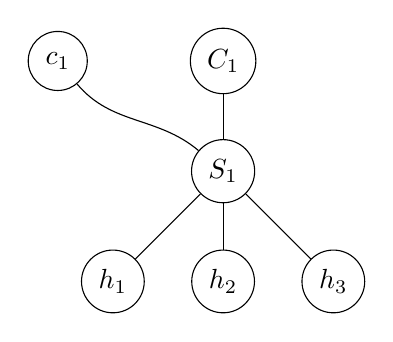
\begin{tikzpicture}[
      every node/.style={draw, circle, minimum width=0.75cm},
      x=0.7cm,
      y=0.7cm]
    \node (c1)    at (-3,  2) {$c_1$};
    \node (ctrl1) at ( 0,  2) {$C_1$};
    \node (S1)    at ( 0,  0) {$S_1$};
    \node (h1)    at (-2, -2) {$h_1$};
    \node (h2)    at ( 0, -2) {$h_2$};
    \node (h3)    at ( 2, -2) {$h_3$};

    \draw (c1) to[out=310,in=140] (S1);
    \draw (S1) -- (ctrl1);
    \draw (S1) -- (h1);
    \draw (S1) -- (h2);
    \draw (S1) -- (h3);

  \end{tikzpicture}
  \caption{A single switch $S_1$ with its controller $C_1$, end-hosts
    $h_1, h_2, h_3$ and one WAN-side client $c_1$.}
  \label{figure:graph.single.switch}
\end{figure}

For an explanation of our nomenclature\index{nomenclature}, we will always
talk about \textit{clients} as being remote hosts on the \ac{WAN} side.

The clients\index{client} are supposed to be placed on the \ac{WAN}---but they are actually
just ordinary hosts on each switch.  We just \textit{pretend} they are
placed on the \acs{WAN}\index{wide-area network}.  It really doesn't matter, though, as all of their
communication goes through each respective switch.

The \textit{end-hosts}\index{end-host} are nodes connected to a single
switch and running services such as key-value stores\index{key-value store},
lock-servers\index{lock-server}, logging servers\index{log server},
databases\index{database}, and so on.

Here is the situation with three switches---the minimum number nodes we need
in a Paxos system.  We have added all-to-all links between the switches in
case any one of them should go down.

\begin{figure}[H]
  \centering
  \begin{tikzpicture}[every node/.style={draw, circle},x=0.7cm,y=0.7cm]
    \foreach \n in {1,2,3} {
      \pgfmathsetmacro\x{(\n-2)*6}
      \node (c\n)    at (\x - 2,  2) {$c_\n$};
      \node (ctrl\n) at (\x ,  2) {$C_\n$};
      \node (S\n)    at (\x ,  0) {$S_\n$};

      \draw (c\n) to[out=305,in=125] (S\n);
      \draw (S\n) -- (ctrl\n);

      \foreach \h in {1,2,3} {
        \pgfmathsetmacro\pos{(\h - 2)*2}
        \pgfmathtruncatemacro\num{((\n - 1)*3) + int(\h)}
        \node (h\num) at (\x + \pos, -2) {$h_{\num}$};
        \draw (S\n) -- (h\num);
      }

    }

    % Links between switches
    \draw (S1) to[out=-10,in=190] (S2);
    \draw (S2) to[out=-10,in=190] (S3);
    \draw [dashed] (S1) to[out=-15,in=195] (S3);

  \end{tikzpicture}
  \caption{Three switches $S_1, S_2, S_3$ with controllers $C_1, C_2, C_3$ acting as Paxos nodes.
           The dashed line between $S_1$ and $S_3$ is a possible \textit{failover-link}.}
  \label{figure:graph.three.switches}
\end{figure}
\todo{Merk at vi kommer til å ha én public IP-adresse for klienter! Så
      må kanskje vise det på en måte (eller bare nevne det)}

The point is that these services will be mirrored by the use of our
Paxos-enabled switches.  For our purposes, we will assume that the services
on these hosts are \textit{deterministic}\index{deterministic}\footnote{Or,
more correctly, \textit{referentially transparent}\index{referential
transparency}.} in the sense that the parameters uniquely determine the
state of the service after being processed---if two hosts running the
same service receive the exact same packet, their state will be
identical after having processed it.  This is a prerequisite for our
system.  The OpenFlow switches, running Paxos, will only make sure that
packets are delivered in the \textit{same order} to the end-hosts.

\section{Viability}

Why would such a system be useful? Consider the situation of implementing
Paxos in code on some servers, running services such as key-value
stores\index{key-value store}, etc.

\begin{figure}[H]
  \centering
  \begin{tikzpicture}[every node/.style={draw, circle},x=0.7cm,y=0.7cm]

    % For each switch ...
    \foreach \n in {1,2,3} {
      \pgfmathsetmacro\x{(\n-2)*6}
      \node (ctrl\n) at (\x ,  2) {$C_\n$};
      \node (S\n)    at (\x ,  0) {$S_\n$};

      \draw (S\n) -- (ctrl\n);

      % For each host ...
      \foreach \h in {1,2,3} {
        \pgfmathsetmacro\pos{(\h - 2)*2}
        \pgfmathtruncatemacro\num{((\n - 1)*3) + int(\h)}

        % Host node
        \node (h\num) at (\x + \pos, -2) {$h_{\num}$};
        \draw (S\n) -- (h\num);

        % Paxos node
        \node [very thick] (P\num) at (\x + \pos, -3.75) {$P$};
        \draw [dashed] (h\num) -- (P\num);
      }
    }

    % Links between switches
    \draw (S1) to[out=-10,in=190] (S2);
    \draw (S2) to[out=-10,in=190] (S3);
    \draw [dashed] (S1) to[out=-15,in=195] (S3);

  \end{tikzpicture}
  \caption{Support for Paxos on the servers $h_1, \dots, h_3$ requires a
    copy of the Paxos code $P$ on each server.}
  \label{figure:paxos.on.servers}
\end{figure}

Here, each server needs to have an implementation of Paxos in code (shown as
$P$ in figure \ref{figure:paxos.on.servers}).  It means the software
developer has to specifically add support for Paxos when designing the
server code, tailoring it for the particular service.  All Paxos handling
must be done at a high networking layer\index{networking layers}---most
likely in the application layer\index{application layer} at the very top.

Now consider the situation where the switch provides Paxos
capabilities\index{Paxos!on switch} (figure \ref{figure:paxos.on.switches}).

\begin{figure}[H]
  \centering
  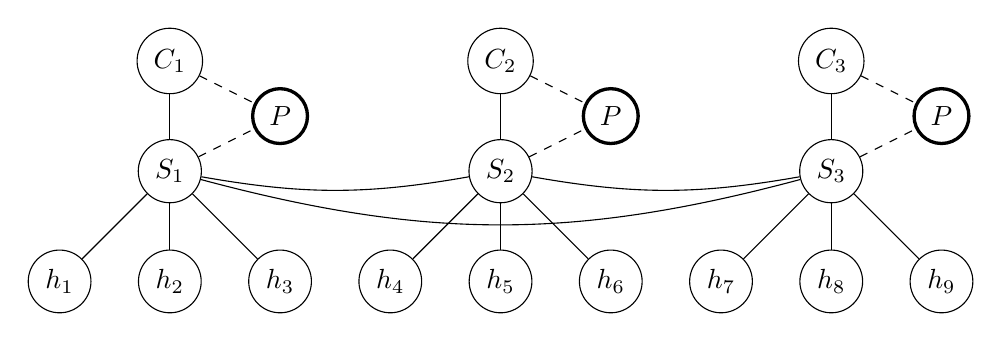
\begin{tikzpicture}[every node/.style={draw, circle},x=0.7cm,y=0.7cm]

    % For each switch ...
    \foreach \n in {1,2,3} {
      \pgfmathsetmacro\x{(\n-2)*6}
      \node (ctrl\n) at (\x ,  2) {$C_\n$};
      \node (S\n)    at (\x ,  0) {$S_\n$};

      \draw (S\n) -- (ctrl\n);

      % Paxos node
      \node [very thick] (P\n) at (\x + 2, 1) {$P$};
      \draw [dashed] (S\n) -- (P\n);
      \draw [dashed] (ctrl\n) -- (P\n);

      % For each host ...
      \foreach \h in {1,2,3} {
        \pgfmathsetmacro\pos{(\h - 2)*2}
        \pgfmathtruncatemacro\num{((\n - 1)*3) + int(\h)}

        % Host node
        \node (h\num) at (\x + \pos, -2) {$h_{\num}$};
        \draw (S\n) -- (h\num);
      }
    }

    % Links between switches
    \draw (S1) to[out=-10,in=190] (S2);
    \draw (S2) to[out=-10,in=190] (S3);
    \draw (S1) to[out=-15,in=195] (S3);

  \end{tikzpicture}
  \caption{Paxos ($P$) on the switches $S_1, S_2, S_3$ mitigates the need for special code on the servers.}
  \label{figure:paxos.on.switches}
\end{figure}

In figure \ref{figure:paxos.on.switches}, the switches themselves (and their
controllers\index{Paxos!controller}) enable
support for Paxos.\footnote{We have moved the servers to several switches
to indicate a distributed nature between the switches.
Paxos on a single switch would not be very useful, as that would be a single
point of failure and---after all---be the sole decision point for message
ordering.}
This should let the servers be oblivious of the fact that Paxos is used to
enable ordering of packet arrival to them.

Besides, Paxos is now run at a much lower networking level\index{networking
layers} and at the point where switching is done---there will be less hops
for each packet.

Of course, there are pros and cons for each scenario.
When implementing Paxos, one can often take advantage of
the particular way each server operates. Sometimes one actually
\textit{needs} to know this to implement Paxos.  Therefore, an
implementation of Paxos in each server's code base would be beneficial.

Also, it means that we need to run code on the switches themselves. This
gives rise to a wide range of non-functional requirements for the code.
For instance, code that runs for too long must be
preempted\index{preemption} to let the switch smoothly handle other
requests. Not doing so may result in packet loss, high latency or
worse---complete incapacity to serve data. Besides, switches do not normally
have hardware capable of running \textit{generic} software fast. They
usually have highly optimized hardware to do some of the heavy-lifting.

On the other hand, in our scenario, we can potentially add support for
message ordering through Paxos on servers that does not already support it.
The kinds of services that this would work on is for systems that are
deterministic in nature: The same input (or client packet) on any server
would produce the same internal state and output.
%
But there is a big class of software that has this behaviour:  Key-value
stores, logging servers, relational databases and so on.\footnote{But not
lock servers, because a lock can only be held by one server at a time.}

The only thing our model does not cover is the situation where a switch goes
completely down.
In that case, each connected server should start
synchronizing their internal state with any of the others that have been up.
\todo{Mangler jo også leader election og failures. Må få
  fram at jeg mener at KONSEPTET støtter mange ting, men ikke vår
    IMPLEMENTASJON.}

All in all, we believe this is a viable experiment with practical benefits.
Indeed, using a software-based approach for switches lets us test our model
on \textit{any} existing piece of server software.

Moreover, we also intend to show how one can optimize the performance of
this model further, by moving parts of the Paxos implementation down into
the switches' flow tables.  This should have a big impact, because Paxos
handling is done at a lower networking layer and closer to the central network
components than what would be the case with Paxos in the server's code.

\todo{Føler vi trenger flere, sterkere argumenter.}
